\documentclass[article]{jss}
\usepackage[utf8]{inputenc}

\providecommand{\tightlist}{%
  \setlength{\itemsep}{0pt}\setlength{\parskip}{0pt}}

\author{
Earo Wang\\Monash University \And Di Cook\\Monash Univeristy \And Rob J Hyndman\\Monash Univeristy
}
\title{Calendar-based graphics for visualising people's daily schedules}

\Plainauthor{Earo Wang, Di Cook, Rob J Hyndman}
\Plaintitle{Calendar-based graphics for visualising people's daily schedules}

\Abstract{
The abstract of the article.
}

\Keywords{calendar-based visualisation, temporal-context data}
\Plainkeywords{calendar-based visualisation, temporal-context data}

%% publication information
%% \Volume{50}
%% \Issue{9}
%% \Month{June}
%% \Year{2012}
%% \Submitdate{}
%% \Acceptdate{2012-06-04}

\Address{
    Earo Wang\\
  Monash University\\
  Department of Econometrics and Business Statistics, Monash University,
  VIC 3800 Australia\\
  E-mail: \email{earo.wang@monash.edu}\\
  
      Di Cook\\
  Monash Univeristy\\
  Department of Econometrics and Business Statistics, Monash University,
  VIC 3800 Australia\\
  E-mail: \email{dicook@monash.edu}\\
  
      Rob J Hyndman\\
  Monash Univeristy\\
  Department of Econometrics and Business Statistics, Monash University,
  VIC 3800 Australia\\
  E-mail: \email{rob.hyndman@monash.edu}\\
  
  }

% Pandoc header

\usepackage{amsmath}

\begin{document}

\section{Introduction}\label{introduction}

Calendar-based visualisation turns out to be a useful tool in unfolding
human-related activities in temporal context. For example,
\citet{VanWijkCluster1999} developed a calendar view of heatmap to
represent the number of employees in the work place over a year, where
colours indicate different clusters derived from the days. It
effectively contrasts weekdays and weekends, highlights public holiday,
and presents other known seasons like school vacations, all of which
have influence over the turn-outs in the office. The calendar-based
heatmap was implemented in a couple of R packages: \texttt{ggTimeSeries}
\citep{R-ggTimeSeries} and \texttt{ggcal} \citep{R-ggcal}. However,
their techniques are too constrained to colour-encoding graphics. We
shall extend this calendar-based arrangement using linear algebra tools
from a single type of heatmap to a broader range of glyphs, from
univariate to multivariate cases, from one calendar format to three
formats. The proposed algorithm has been developed in the
\texttt{sugrrants} package \citep{R-sugrrants} using R \citep{R-base}.

This work was originally motivated by studying hourly foot traffic in
the city of Melbourne \citep{ped}. There have been 43 sensors installed
across downtown Melbourne since 2009 in order to capture the pulse of
city life. (FIGURE ?: weekday at multiple sensors) Figure (?) lends
itself to addressing some of the issues:

\begin{enumerate}
\def\labelenumi{\arabic{enumi}.}
\tightlist
\item
  to simultaneously exhibit multiple seasons including time of day, day
  of week, and day of year
\item
  to visualise long historical time series data in an information-dense
  way at the overview level
\item
  to compare and contrast multiple time series on a common scale
\item
  to quickly look up the date when there are unexpected events happening
  without interactivity.
\end{enumerate}

\section{The function and its
construction}\label{the-function-and-its-construction}

In the section, the algorithms to construct calendar grids, different
scales, and reference lines and labels are discussed in detail.

\begin{verbatim}
frame_calendar(
  data, x, y, date, calendar = "monthly", dir = "h", sunday = FALSE, 
  nrow = NULL, ncol = NULL, polar = FALSE, scale = "fixed"
)
\end{verbatim}

\subsection{Grid construction}\label{grid-construction}

The algorithm for constructing a calendar plot uses linear algebra,
similar to that used in the glyph map displays for spatio-temporal data
\citep{Wickham2012glyph}. To make a year long calendar, requires cells
for days, embedded in blocks corresponding to months, organised into a
grid layout for a year. Each month can be captured with 35 (5 \(\times\)
7) cells, where the top left is Monday of week 1, and the bottom right
is Sunday of week 5. These cells provide a micro canvas on which to plot
the data. The first day of the month could be any of Monday-Sunday,
which is determined by the year of the calendar. Months are of different
length days, ranging form 28-31, and each month could extend over six
weeks but the convention in these months is to wrap the last few days up
to the top row of the block. The notation for creating these cells is as
follows:

\begin{itemize}
\tightlist
\item
  \(k = 1, \dots , 7\) is the day of the week that is the first day of
  the month
\item
  \(d = 28, 29, 30\) or \(31\) representing the number of days in any
  month
\item
  \((i, j)\) is the grid position where \(1 \le i \le 5\) is week within
  the month, \(1 \le j \le 7\), is day of the week.
\item
  \(g = k, \dots,(k+d)\) indexes the day in the month, inside the 35
  possible cells
\end{itemize}

The grid position for any day in the month is given by

\begin{equation}
  \begin{aligned}
  i &= \lceil (g \mod 35) / 7\rceil, \\
  j &= g \mod 7. \label{eq:grid}
  \end{aligned}
\end{equation}

Figure \ref{fig:month-diagram} illustrates this \((i,j)\) layout for a
month where \(k=5\).

\begin{CodeChunk}
\begin{figure}

{\centering 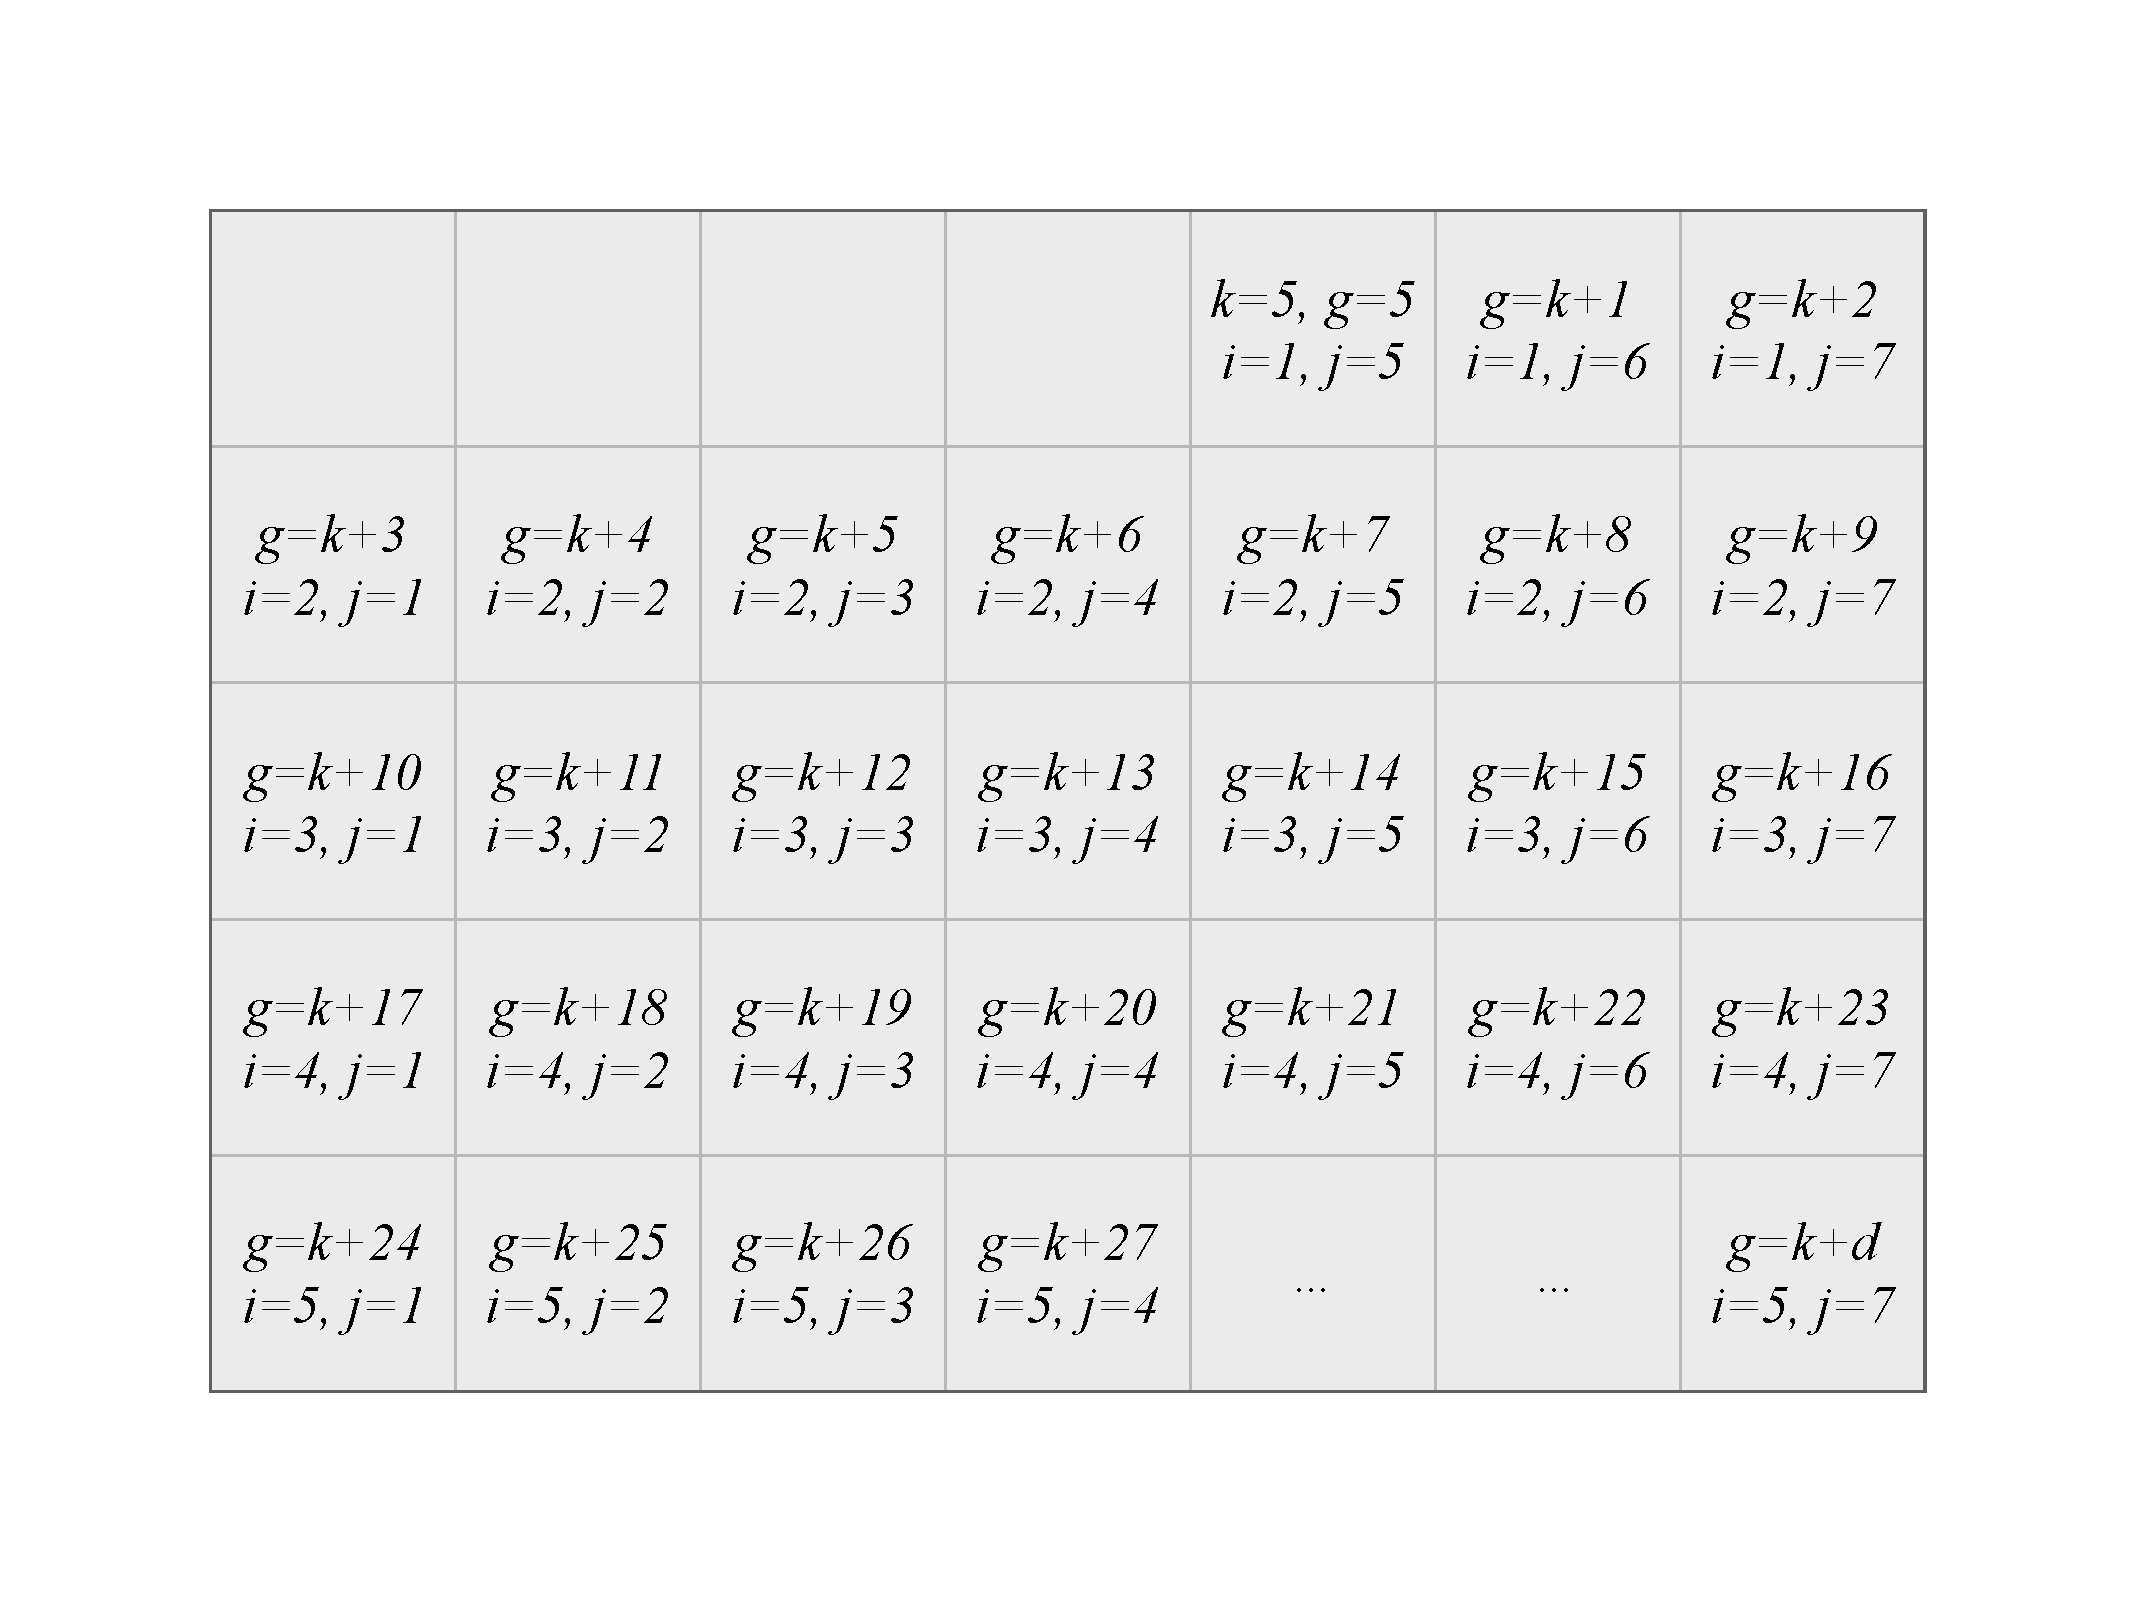
\includegraphics[width=360pt,height=250pt]{figure/month} 

}

\caption[Illustration of the indexing layout for cells in a month]{Illustration of the indexing layout for cells in a month.}\label{fig:month-diagram}
\end{figure}
\end{CodeChunk}

To create the layout for a full year, \((m, n)\) denotes the position of
the month arranged in the plot, where \(1 \le m \le M\) and
\(1 \le n \le N\). Between each month requires some small amount of
white space, label this \(b\). Figure \ref{fig:year-diagram} illustrates
this layout.

\begin{CodeChunk}
\begin{figure}

{\centering 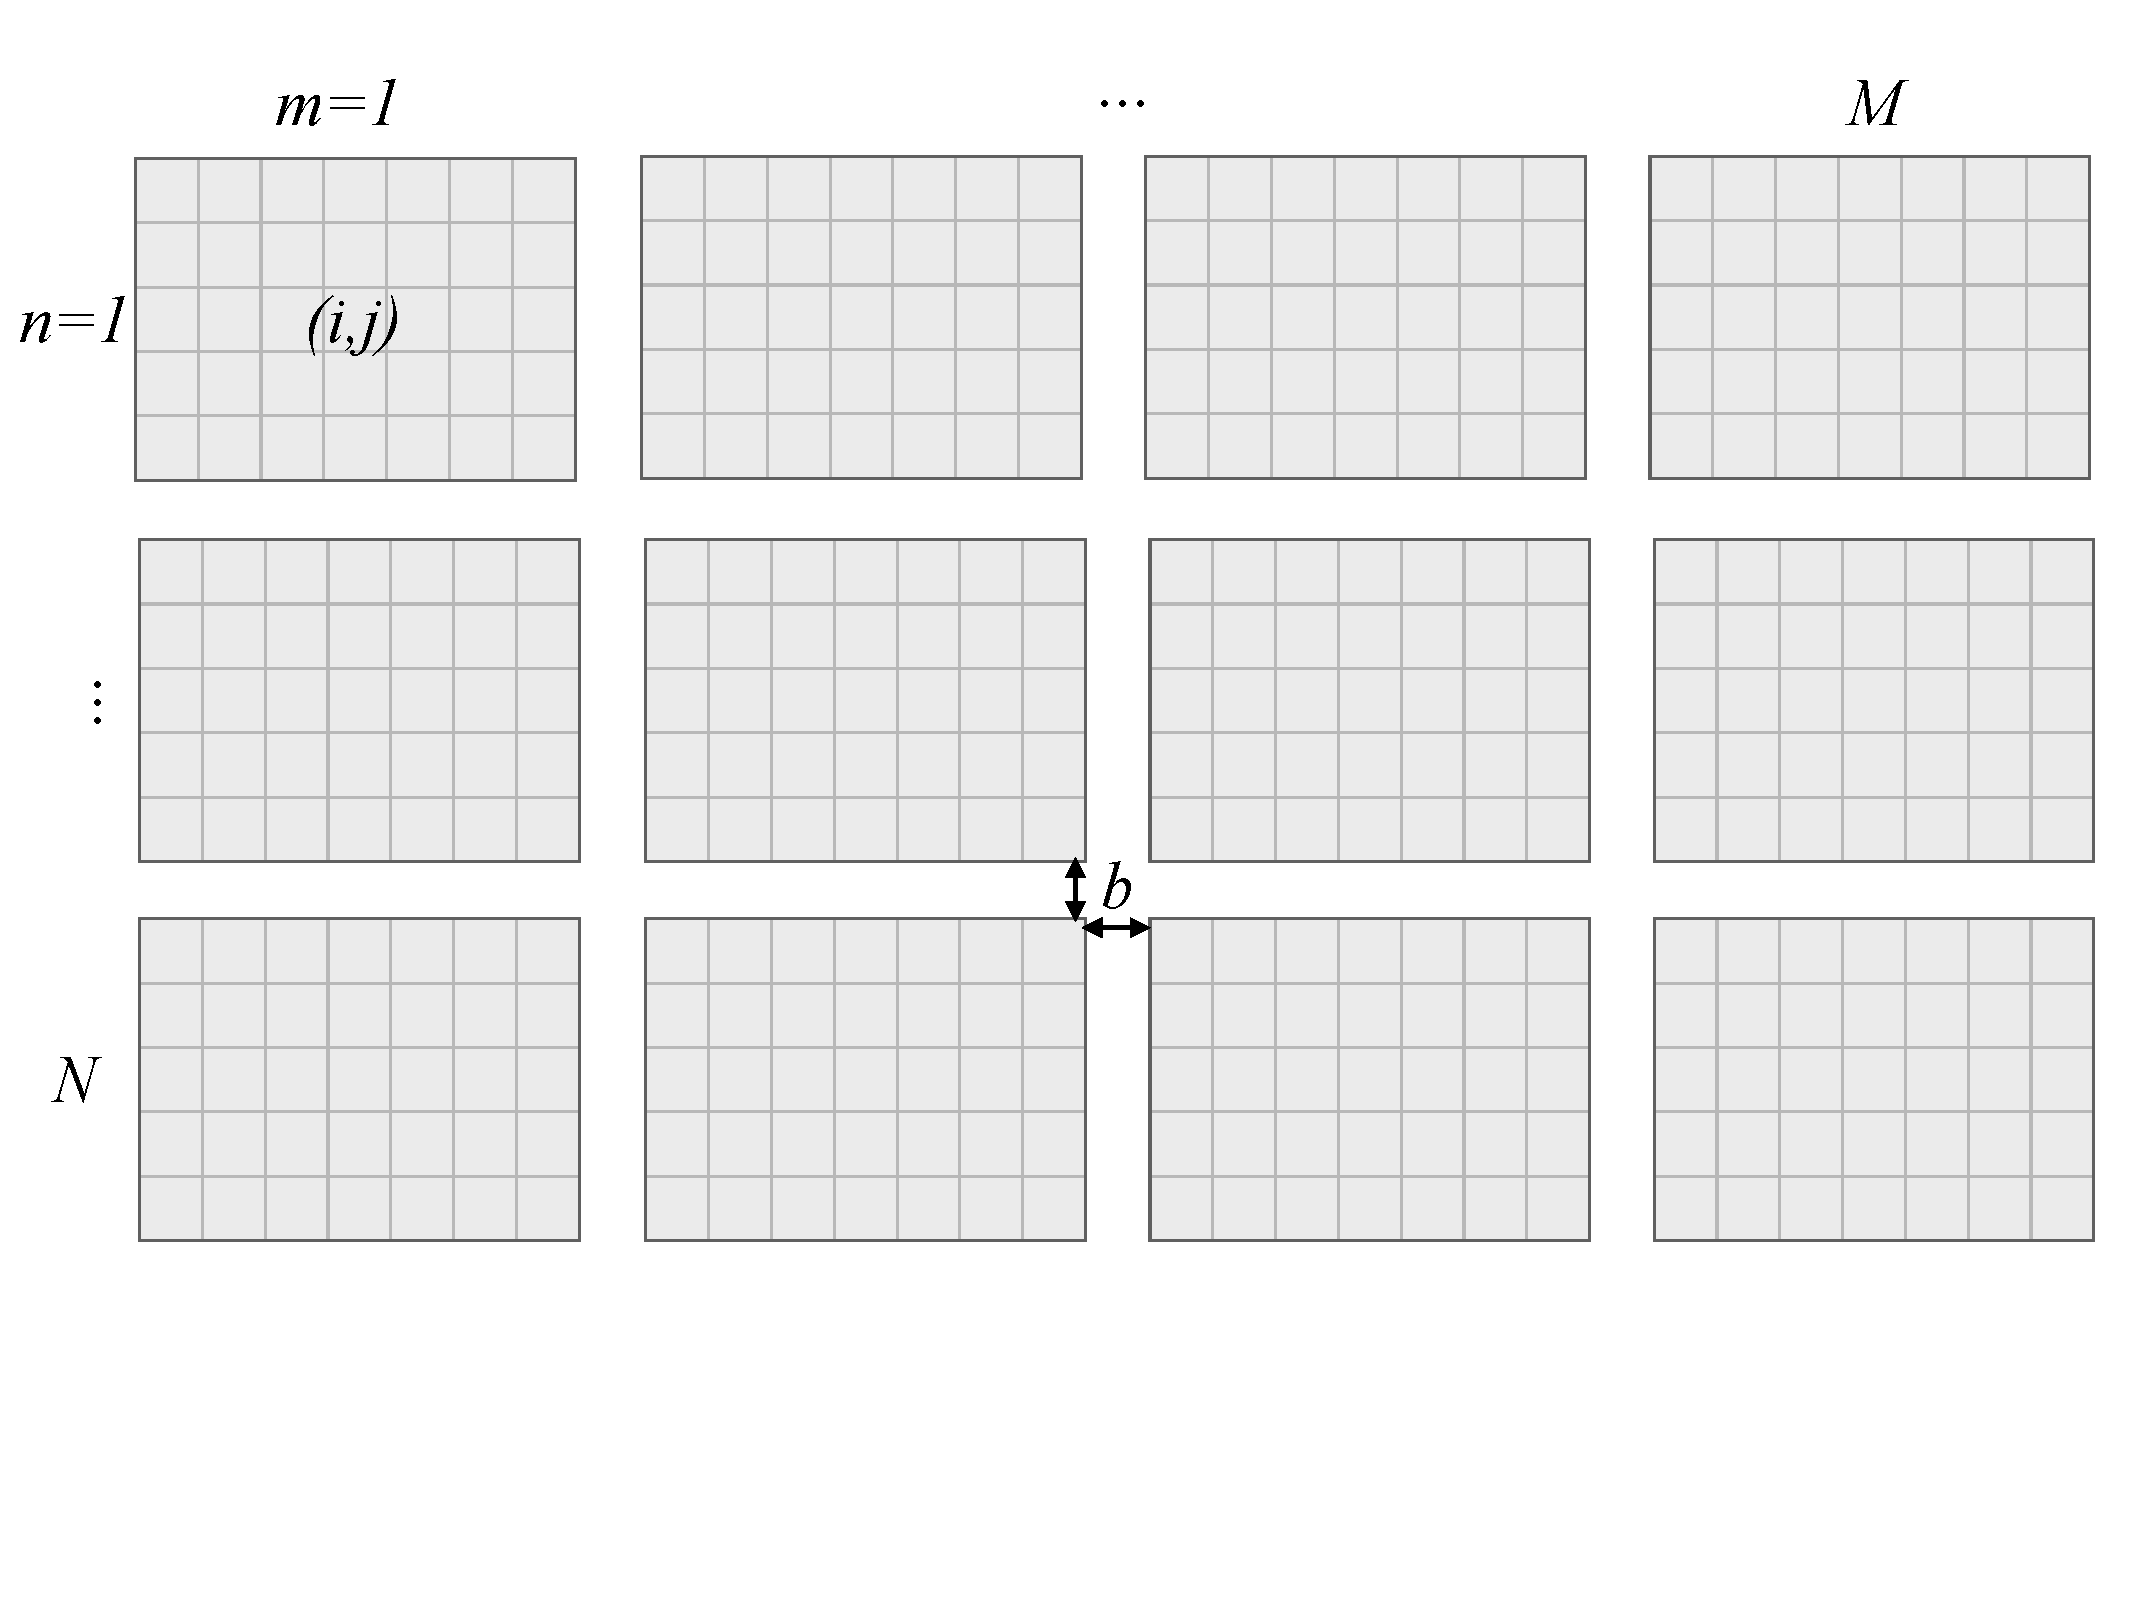
\includegraphics[width=360pt,height=250pt]{figure/year} 

}

\caption[Illustration of the indexing layout for months of one year]{Illustration of the indexing layout for months of one year.}\label{fig:year-diagram}
\end{figure}
\end{CodeChunk}

Each cell forms a canvas on which to draw the data. Consider the canvas
to have limits \([0, 1]\) horizontally and vertically. For the
pedestrian sensor data, within each cell hour is plotted horizontally
and count is plotted vertically. Each variable is scaled to have values
between \([0,1]\), using the minimum and maximum of all the data values
to be displayed. Let \(h\) be the scaled hour, and \(c\) the scaled
count.

Then the final points for making the calendar line plots of the
pedestrian sensor data is given by:

\begin{equation}
  \begin{aligned}
  x &= i + (i - 1) \times m + (m - 1) \times b + h, \\
  y &= -j - (j - 1) \times n - (n - 1) \times b + c. \label{eq:final}
  \end{aligned}
\end{equation}

Note that for the vertical direction, the top left is the starting point
of the grid, hence the subtractions, and resulting negative values to
lay out the cells. Within each cell, the starting position is bottom
left.

The algorithm can be extended relatively easily to layout from one
single month to multiple years depending on the time span to be
visualised. The month-by-month arrangement can be determined by the
user's choice through \(M\) and \(N\). If one would like to compare and
contrast January, February and so on across multiple years, \(M = 12\)
and \(N\) depending on the number of years could be setup.

Monthly calendar format provides an effective layout to emphasise
differences between weekdays and weekends as well as day of year (for
example, public holiday) simultaneously, however, either one of which is
sufficient in certain visualisation applications. If there is apparent
depiction of weekday effects but none of yearly effects, weekly calendar
format (weeks of a year) could be considered employing; otherwise days
of a month could be laid out for standing-out yearly behaviours.

(MAKE TWO DIAGRAMS ON WEEKLY AND DAILY CALENDAR FORMATS IN KEYNOTE).
Weekly and daily calendar formats are the simplifications of monthly
calendar.

We only illustrate that calendar grids are laid out on the horizontal
direction. The vertical direction can be enabled by swapping \(i\) and
\(j\) in the algorithm stated above. It is useful for users in some
countries where they get used to calendars of vertical organisation and
other possible comparisons like Mondays across the columns rather than
rows.

\subsection{Scales}\label{scales}

One of the advantages using glyphs over heatmaps is evident in easily
enabling scales on different temporal scales. All of the line glyphs
shown above are drawn on the global scale so that it makes the
magnitudes comparable over all the period. On the other hand, some
sub-series of small magnitudes yet worth-noting shapes possibly become
invisible whilst embedded in the overall picture. The individual scale
or something else, as a result, complements the calendar-based
visualisation in general.

There are other three types of scales in addition to the global scale:
individual scales regardless of days, conditional on weekdays, and
conditional on days of a month.

\subsection{Reference lines and
labels}\label{reference-lines-and-labels}

It can be noted that reference lines separating each cell and panel and
labels indicating weekday and month are also constructed in order to
make calendar-based graphics more accessible and informative.

Regarding the monthly calendar format, the major reference lines
separate every month panel and the minor ones separate every day cell,
represented by the think and thin lines respectively. The major
reference lines are placed on the far left and right as well as the
bottom and top of every month panel: for each \(m\), the vertical lines
are determined by \(\min{(x)}\) and \(\max{(x)}\); for each \(n\), the
horizontal lines are computed by \(\min{(y)}\) and \(\max{(y)}\). The
minor reference lines are placed on the initial positions: for each
\(i\), the vertical line is \(\min{(x)}\); for each \(j\), the
horizontal line is \(\min{(y)}\).

The abbreviated month labels located on the top left are obtained
through \((\min{(x)}, \max{(y)})\) for every \(m\) and \(n\). The
weekday texts with a single letter are uniformly placed on the bottom of
the whole canvas, that is \(\min{(y)}\).

\section{Examples}\label{examples}

\section{Discussion}\label{discussion}

The calendar-based visualisation provides data plots in the familiar (at
least for the Western world) format of an everyday tool. Special events
for the region, like Anzac Day in Australia, or Thanksgiving Day in the
USA, more easily pop out to the viewer as public holidays, rather than a
typical work day.

This sort of layout may be useful for studying consumer trends, or human
behaviour, like the pedestrian patterns. It may not work so well for
physical patterns like temperature, which are not typically affected by
human activity.

The limitation is also evident: hard to perceive trend as not on the
common scale.

We shall enable interactivity in the calendar-based graphics for time
series data. It will allow users to transform different temporal
components and switch displays between overlaying and faceting through
key strokes or mouse clicks.

\bibliography{packages.bib,references.bib}


\end{document}

